\documentclass[a4paper]{article}

%%%%%%%%%%%%%%%%%%%%%%%%%%%%%%%%%%%%%%%%%%%%%%
% Gestion du français et des accents %
\usepackage[utf8x]{inputenc}
\usepackage[T1]{fontenc}
\usepackage[greek, french]{babel}
%%%%%%%%%%%%%%%%%%%%%%%%%%%%%%%%%%%%%%%%%%%%%%

%%%%%%%%%%%%%%%%%%%%%%%%%%%%%%%%%%%%%%%%%%%%%%
% Gestion des Sections et de la Table des matières %
\setcounter{secnumdepth}{3}
\setcounter{tocdepth}{3}

\usepackage[]{titletoc}
%\titlecontents
%		{section}
%		[left]
%		{au-dessus}
%		{avant (si label)}
%		{avant (sans label)}
%		{remplissage et n°page}
%		[après]



%%%   Section   %%%

\titlecontents
	{section}
	[25pt]
	{\addvspace{0.75pc}}
	{\normalfont\scshape\contentslabel{25pt}}
	{}
	{\normalsize\hfill\bfseries ~\thecontentspage\vspace{-3pt}\hrule}
	[\addvspace{0.5pc}]
	


%%%   Sous-Section   %%%

\titlecontents
	{subsection}
	[75pt]
	{\addvspace{-0.5pc}}
	{\normalfont\small\contentslabel{30pt}}
	{}
	{\normalsize\dotfill\small\thecontentspage}
	[]



%%%   Sous-sous-Section   %%%

\titlecontents
	{subsubsection}
	[125pt]
	{\addvspace{-0.5pc}}
	{\normalfont\footnotesize\contentslabel{30pt}\itshape}
	{}
	{\normalsize\hfill\footnotesize\itshape\thecontentspage}
	[]
	
\contentsfinish
%%%%%%%%%%%%%%%%%%%%%%%%%%%%%%%%%%%%%%%%%%%%%%

%%%%%%%%%%%%%%%%%%%%%%%%%%%%%%%%%%%%%%%%%%%%%%
% Gestion des marges du document %

\usepackage{geometry}

\geometry{
paperwidth=21cm,
%width=15.5cm,
left=3cm,
right=3cm,
paperheight=29.7cm,
%height=26.5cm,
top=3cm,
bottom=3cm,
headheight=0cm,
headsep=0cm,
footskip=1cm
}
%%%%%%%%%%%%%%%%%%%%%%%%%%%%%%%%%%%%%%%%%%%%%%

\usepackage{graphicx}
\usepackage{setspace}
\usepackage{mathtools}
\usepackage{rotating}
\usepackage{multirow}
\usepackage{multicol}
\usepackage{Tkz-Tab}
\usepackage{makecell}

%\usepackage[mathletters]{ucs}

\DeclareFontEncoding{LS1}{}{}
\DeclareFontSubstitution{LS1}{stix}{m}{n}
\DeclareSymbolFont{symbols4}{LS1}{stixbb}{m}{it}
\DeclareMathSymbol{\varhexagonblack}{\mathord}{symbols4}{"DD}
\DeclareMathSymbol{\hexagonblack}   {\mathord}{symbols4}{"DE}


\usepackage{setspace}
\usepackage{amssymb}
\usepackage{numprint}

\def\nbR{\ensuremath{\mathrm{I\! R}}}


\renewcommand{\thesection}{\Roman{section}}
\renewcommand{\thesubsubsection}{\roman{subsubsection}}

\usepackage{xlop}
\usepackage{ulem}

\parindent=1cm

\usepackage[bottom]{footmisc}
\usepackage[dvipsnames]{xcolor}

\usepackage{footnote}
\makesavenoteenv{tabular}

\begin{document}

	\begin{titlepage}
		\begin{center}
		
			\Huge	 \textbf{Recueil de Mathématiques}\\
			\bigskip \smallskip
		
			\Large	 \textbf{$\varhexagonblack$ Section 3 - Trigonométrie $\varhexagonblack$}\\
			\bigskip
		
			\large	 Clément \sc{Campana}  \\ 
			\smallskip
		
			\normalfont Février 2024 \\
		
		\end{center}
		
		%\onehalfspacing
		\doublespacing
		\tableofcontents
		\singlespacing

	\end{titlepage}




% -------------------------------------------------------------

	\section{Premier pas en Trigonométrie}

		La Trigonométrie est, comme son nom l'indique, une discipline mathématique qui a comme objectif de "mesurer" les triangles.

		Plus clairement, son but est de pouvoir déduire l'ensemble des informations disponibles dans un 
		triangle à partir du minimum d'information sur ce triangle.
		Comme vu dans la Section 2, un triangle est un polygone à 3 côtés, 
		et la somme des 3 angles d'un triangle vaut 180°, $\pi$ rad ou 200 gr.

		En général, en Trigonométrie, on se focalise principalement sur les \textit{triangles rectangles}, 
		puis on généralise les théorèmes que nous avons démontré à tous les triangles.

		\subsection{Construction d'un triangle}
	
			Les triangles ont une particularité les différenciant des autres polygones :

			\textbf{En connaissant la longueur de 3 côtés d'un triangle, il est possible de parfaitement construire ce triangle.}

			Dans les autres polygones, cette condition n'est pas suffisante pour le construire\footnote{
				Par exemple, si l'on prend un quadrilatère donné, 
				où l'on a fixé la longueur de 4 côtés,
				il est possible de "l'écraser" afin d'obtenir un autre
				quadrilatère ayant les mêmes longueurs de côtés.
				En revanche, les angles formés par les côtés de ce quadrilatère 
				ne seront pas les mêmes que ceux du quadrilatère de départ.
				
				~~Ainsi, à partir d'un losange, il est possible de créer un carré, 
				en fonction des angles choisis entre les côtés.

				~~~Pour la même raison, 
				les polygones ayant plus de côtés ne sont pas constructibles
				en connaissant uniquement les longueurs de leurs côtés.
			}.

			\medbreak

			Pour tracer un triangle à l'aide de \textit{trois longueurs}, 
			il faut tracer un segment mesurant une des trois longueurs choisies, 
			puis tracer deux cercle ayant comme centre les extrémités du segment 
			et comme rayons les deux autres longueurs voulues pour le triangle. 
			Les cercles se croisent en deux points, 
			avec lesquelles ont peut construire deux triangles symétriques.

			\medbreak

			Mais l'on peut aussi remplacer un des cercles ou les deux 
			cercles par une ou des demi-droites, 
			ayant un angle interne d'une valeur choisie. 
			Cette demi-droite et le cercle ou ces deux demi-droites 
			vont se croiser en un point, le troisième sommet du triangle.

			Voici un tableau récapitulatif des différentes possibilités de construction d'un triangle, 
			en fonction du nombre d'informations connues sur celui-ci :

			\begin{center}
					\renewcommand{\arraystretch}{1.25}
					\begin{tabular}{|c|c|c|c|c|}
						\hline
									           & \textbf{Aucune longueur}         & \textbf{1 longueur}              & \textbf{2 longueurs}             & \textbf{3 longueurs}             \\
						\hline
						\textbf{Aucun angle}   & \textcolor{Red}{Inconstructible} & \textcolor{Red}{Inconstructible} & \textcolor{Red}{Inconstructible} & \textcolor{Green}{Constructible} \\
						\hline
						\textbf{1 angle}       & \textcolor{Red}{Inconstructible} & \textcolor{Red}{Inconstructible} & \textcolor{Green}{Constructible} & \textcolor{Green}{Constructible} \\
						\hline
						\textbf{2 ou 3 angles}\footnote{
							En connaissant deux angles d'un triangle, 
							il est possible de déduire le troisième, 
							car la somme des trois angles d'un triangle 
							correspond à un angle plat.
											} & Triangles semblables\footnote{
											Avec deux ou trois angles, 
											il n'est pas possible de construire un triangle en particulier,
											mais seulement une collection de triangles semblables entre-eux.
										}& \textcolor{Green}{Constructible} & \textcolor{Green}{Constructible} & \textcolor{Green}{Constructible} \\
						\hline
					\end{tabular}
			\end{center}

			Nous pouvons en conclure qu'un triangle en particulier, 
			est traçable à l'aide d'une longueur et de deux autres mesures 
			(des angles ou des longueurs).

			\begin{center}
				\makebox[\textwidth][c]{
					\begin{tabular}{cc}
						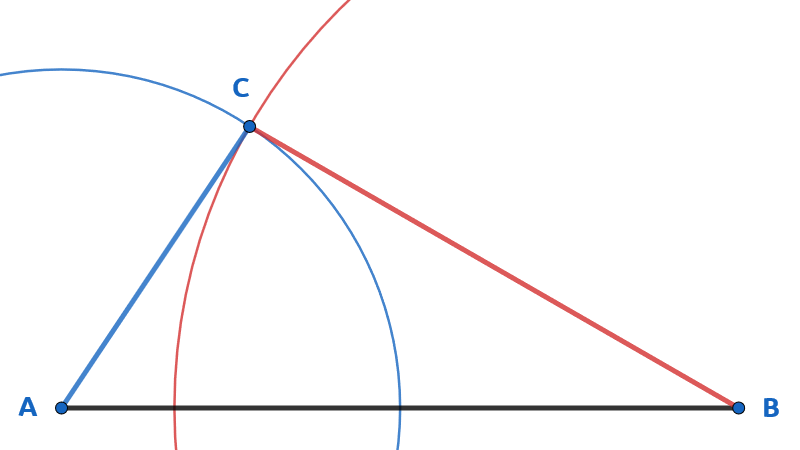
\includegraphics[width=7cm]{Image/Triangle/Triangle_construction_3_longueurs.png}         &
						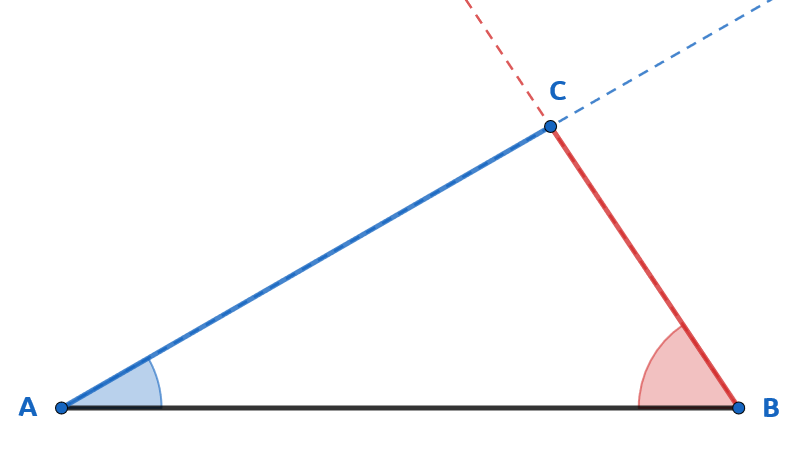
\includegraphics[width=7cm]{Image/Triangle/Triangle_construction_1_longueur_2_angles.png} \\

						\textit{Triangle construit avec 3 longueurs} & \textit{Triangle construit avec 1 longueur et 2 angles} \\
					\end{tabular}
				}
			\end{center}

			Cette propriété unique aux triangles, nous sera très utile par la suite.

			\medbreak


\newpage
		
		\subsection{Fonctions trigonométriques}

		\subsubsection{Relation entre les longueurs des côtés d'un triangle rectangle}

			Prenons un triangle rectangle, 
			dont (par définition) nous connaissons un des angles, 
			son angle droit (qui vaut 90°, $\frac{\pi}{2}$ rad ou 100 gr).

			Prenons un autre de ces angles, que nous appellerons $\alpha$. 
			
			Nous connaissons ainsi deux angle, l'angle droit et l'angle $\alpha$.
			Comme nous savons que la somme des trois angles du triangle vaut un angle plat,
			nous pouvons déduire la mesure du dernier angle.
			Notre troisième angle (que nous nommerons $\beta$) vaut en degré : $\beta = 180^\circ - (90^\circ + \alpha) = 90^\circ - \alpha$

			\medbreak

			Maintenant, nous avons obtenues les mesures des trois angles du triangle.
			Comme vu plus précédemment dans le tableau,
			avec uniquement 3 angles, il est possible de construire une collection de \textbf{triangles tous semblables entre-eux}.

			Afin d'être plus clair, nommons les côtés de notre triangle $a$, $b$ et $c$, en fonction de leur taille.
			Le côté $a$ sera le plus court, le côté intermédiaire sera le $b$ et le plus long sera le $c$.

			\medbreak

			Prenons deux de triangles de cette collection, le triangle 1 et le triangle 2. 
			Leurs côtés mesures $a_1$, $b_1$, $c_1$ et $a_2$, $b_2$, $c_2$.
			Comme ces triangles sont semblables, 
			leurs côtés sont proportionnels entre-eux,
			ce qui signifie que $\frac{a_1}{a_2} = \frac{b_1}{b_2} = \frac{c_1}{c_2}$.

			Cette propriété implique que, les rapports entre les côtés dans un triangle 
			vont être égaux à ceux des mêmes côtés dans un autre triangle semblable au premier.

			\medbreak

			Mathématiquement, cela signifie que, 
			pour les côtés $a$ et $b$ de deux triangles semblables, 
			on a $\frac{a_1}{b_1} = \frac{a_2}{b_2}$.

			Démontrons cette propriété :
			$\frac{a_1}{a_2} = \frac{b_1}{b_2}$
			$\Longleftrightarrow a_1 \times b_2 = a_2 \times b_1$
			$\Longleftrightarrow \frac{a_1 \times b_2}{b_1} = a_2$
			$\Longleftrightarrow \frac{a_1}{b_1} = \frac{a_2}{b_2}$

			Les démonstrations des relations entre les autres côtés sont analogues.

			\medbreak

			Cela signifie que les \textbf{rapports entre les longueurs} des côtés dans triangle, ne dépend que des mesures des angles.

			De plus, comme nous sommes dans un triangle rectangle,
			tous les angles du triangle sont soit fixé à l'avance (l'angle droit), 
			ou ne dépendent que de la mesure de l'angle $\alpha$. 

			\medbreak

			Et enfin, 
			nous pouvons en conclure que les rapports entre tous les côtés d'un triangle rectangle,
			ne dépendent que de la mesure de l'angle $\alpha$.

			\bigbreak
			\bigbreak

		\subsubsection{Définition des fonctions trigonométriques élémentaires}

			Comme montré plus tôt, les rapports en chaque côté d'un triangle rectangle, 
			ne dépendent que de l'angle $\alpha$ (défini comme étant un autre angle que l'angle droit).
			
			En revanche, ce rapport entre longueurs n'est pas simplement constant, 
			il varie de manière complexe en fonction de l'angle $\alpha$.
			
			\medbreak

			Pour prendre en compte ces variations, et donc pouvoir obtenir une relation chiffrée, 
			les mathématiciens ont construits un grand arsenal de fonctions trigonométriques\footnote{
				Une grande partie des fonctions trigonométriques créées sont rarement utiles, 
				pour en savoir plus sur ces fonctions délaissées, rendez-vous en Annexe, à la page \pageref{fonction_trigo_chelous}.
			}. 
			

			{\noindent Les fonctions trigonométriques les plus utiles sont : }
			
			\begin{itemize}
				\item [•] La fonction \emph{sinus}, notée $\sin$.
				\item [•] La fonction \emph{cosinus}, notée $\cos$.
				\item [•] La fonction \emph{tangente}, notée $\tan$.
			\end{itemize}

			\bigskip

			{\noindent Dans ces relations, on utilise : }
			
			\begin{itemize}
				\item [•] L'angle $\alpha$, définit précédemment.
				\item [•] La cathète opposée à l'angle $\alpha$ (noté $O$ et généralement appelée "côté opposé").
				\item [•] La cathète adjacente à l'angle $\alpha$ (noté $A$ et généralement appelée "côté adjacent").
				\item [•] L'hypoténuse du triangle (noté $H$).
			\end{itemize}

\newpage

			Voici les relations en questions, qui sont les définitions respectives de la fonction sinus, cosinus et tangente :
			
			\begin{center}
				
				%\renewcommand{\arraystretch}{3ex}
				\setcellgapes{2.5mm}
				\makegapedcells
				\begin{tabular}{|c|ccc|}
					\hline
					\textbf{Fonction} & \textbf{Définition}                                                                 & \multicolumn{2}{c|}{\textbf{Résumé}} \\
					\hline
					\textbf{Sinus}    & $\sin(\alpha) =$ {\Large $\frac{\text{Cathète Opposée}}{\text{Hypoténuse}}$       } & $\sin(\alpha) = \frac{\text{O}}{\text{H}} \Longrightarrow \text{S = O / H} $ & \textit{SOH} \\
					\textbf{Cosinus}  & $\cos(\alpha) =$ {\Large $\frac{\text{Cathète Adjacente}}{\text{Hypoténuse}}$     } & $\cos(\alpha) = \frac{\text{A}}{\text{H}} \Longrightarrow \text{C = A / H} $ & \textit{CAH} \\
					\textbf{Tangente} & $\tan(\alpha) =$ {\Large $\frac{\text{Cathète Opposée}}{\text{Cathète Adjacente}}$} & $\tan(\alpha) = \frac{\text{O}}{\text{A}} \Longrightarrow \text{T = O / A} $ & \textit{TOA} \\
					\hline
				\end{tabular}
			\end{center}

			Un bon moyen mnémotechnique pour retenir ces définitions, 
			est l'expression "\textit{Casse-toi !}". 
			On peut l'obtenir en utilisant les résumés des définitions à droite, 
			réarrangeant les définitions, en mettant celle du cosinus en premier.
			Ainsi, on obtient "\textit{CAH, SOH, TOA}".
			
			\medbreak

			A l'aide de ces relations, 
			il est possible de connaître toutes les longueurs de 
			tous les côtés d'un triangle rectangle à l'aide uniquement 
			de la mesure d'un de ses angles et d'une longueur d'un des côtés.

			
			
			\begin{center}
				\renewcommand{\arraystretch}{1.75}
				\begin{tabular}{lc|c|c|cc}
					\multicolumn{5}{l}{Exemple :} & \multirow{3}{*}{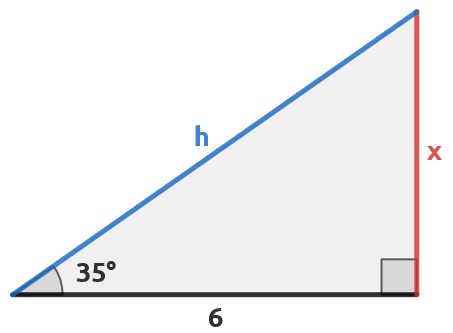
\includegraphics[height=2.5cm]{Image/Triangle/Triangle_sinus_cosinus.png}} \\
					
					\phantom{Exemp} & \textit{CAH} & $\text{C = A / H}$ & $\cos(35^\circ) = \frac{6}{h}$ & $h = \frac{6}{\cos(35^\circ)} \approx 7,32 $ & \\
										& \textit{TOA} & $\text{T = O / A}$ & $\tan(35^\circ) = \frac{x}{6}$ & $x = 6 \times \tan(35^\circ) \approx 4,20 $ &\\
				\end{tabular}
			\end{center}
			

			\vfill



		\subsubsection{Lien entre ces trois fonctions} \label{lien_fct_trigo}

			De plus,
			il est possible d'établir un lien entre ces trois fonctions\footnote{Cette relation n'est vraie que si le dénominateur n'est pas nul. 
			
			~~Ainsi si $\alpha \equiv \frac{\pi}{2} [\pi] $, c'est à dire si $\exists k \in \mathbb{Z},\alpha = k\pi + \frac{\pi}{2}$, la tangente de cet angle n'est pas définie.} :
			{ \Large $$ \tan(\alpha) = \frac{\sin(\alpha)}{\cos(\alpha)} $$}

			\medbreak
			\medbreak

			Pour démontrer cette relation, 
			on peut utiliser la définition de la tangente, 
			puis remplacer les longueurs des côtés à l'aide 
			des définitions des fonctions sinus et cosinus :

			\medbreak

			\begin{itemize}
				\item [ ] $\text{Cathète Opposée}   = \sin(\alpha) \times \text{Hypoténuse}$
				\item [ ] $\text{Cathète Adjacente} = \cos(\alpha) \times \text{Hypoténuse}$
			\end{itemize}

			\bigbreak

			\begin{Large}
			\begin{itemize}
				\item [ ] $\tan(\alpha) = \frac{\text{Cathète Opposée}}{\text{Cathète Adjacente}} = \frac{\sin(\alpha) \times \text{Hypoténuse}}{\cos(\alpha) \times \text{Hypoténuse}} = \frac{\sin(\alpha)}{\cos(\alpha)}$
			\end{itemize}
			\end{Large}

			\vfill

\newpage

	\section{Cercle trigonométrique}

		\subsection{Unité d'angle reine en Trigonométrie : le radian}

			Comme présenté dans la Section 2, 
			il existe plusieurs unités d'angle différentes.

			L'unité la plus utilisée est le degré, 
			mais cette dernière n'est pas la plus adaptée 
			en mathématique, en particulier en Trigonométrie,
			où l'on préfère utiliser le radian.

			Pour en savoir plus sur les définitions des unités d'angle,
			rendez-vous dans la Section 2, dans la partie consacrée aux Angles.

			\subsubsection*{Rappel de la définition du radian}

				Pour un angle donné, 
				la mesure en radians de cet angle est égale 
				à la longueur de l'arc de cercle intercepté par cet angle,
				sur un cercle de rayon 1.

				Ainsi, le radian est l'unité étant la plus cohérente mathématiquement,
				car elle est basée sur la longueur de l'arc de cercle formé.
				Cette cohérence a donné à cette unité un statut privilégié\footnote{
					Au premier abord, 
					le statut privilégié du radian ne semble pas solidement justifiée.
					C'est à dire que, mis à part la \textit{beauté mathématique} 
					de la définition du radian par rapport au degré, 
					pourquoi cette unité est à préférer à une autre ?
					
					~~Cette préférence provient de certaines propriétés mathématiques 
					qui ne sont vrai que si l'unité d'angle est le radian.
					En particulier, lorsque l'on dérive ou intègre une 
					fonction trigonométrique ou encore lorsque 
					l'on utilise un développement limité de 
					cette fonction trigonométrique.
					Dans ces cas, l'angle peut se retrouver en facteur, 
					position où seule la mesure en radians d'un angle a un sens.
				} en mathématique, en particulier en Trigonométrie.

				Cependant, le périmètre d'un cercle étant égal à $2 \pi$, 
				on retrouve la constante $\pi$ un peu partout 
				dans les mesures d'angles usuels. 
				Cette constante rend l'utilisation 
				de cette constante peu intuitive, 
				ce qui explique certainement pourquoi cette unité, 
				mathématiquement meilleure que le degré, 
				ne s'est pas imposée au plus grand nombre 
				comme remplaçante de cette vielle unité.

				Et c'est pour cette raison que,
				par défaut, c'est cette unité qui sera 
				utilisée à partir de maintenant.

			
		\subsection{Cercle trigonométrique}

			Pour représenter des angles et 
			bien comprendre leur lien avec 
			les fonctions trigonométriques, 
			on utilise généralement le \emph{cercle trigonométrique}. 
			Ce cercle est centré autour de l'origine 
			du repère et à un rayon égal à 1 :

			\begin{multicols}{2}

				\begin{center}
					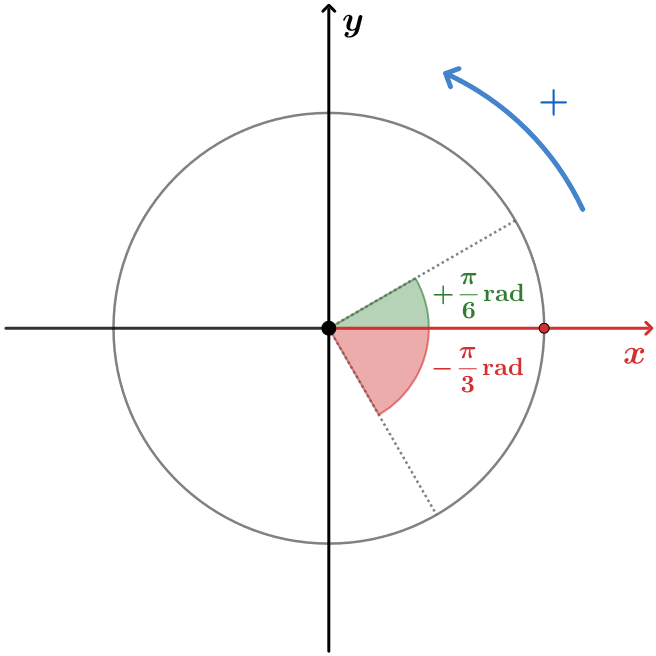
\includegraphics[height=7.2cm]{Image/Cercle Trigo/Cercle_trigo_sens_trigo.PNG}
					\vspace{0.25cm}
				\end{center}

				Les angles représentés sur ce cercle sont \emph{orientés},
				c'est-à-dire qu'ils démarrent à partir d'une ligne et qu'il se terminent sur une autre ligne.
				
				Leur orientation est indiqué par la flèche en haut à droite du cercle, 
				ce sens, inverse au sens dans lequel tournent les aiguilles d'une montre, 
				est appelé \emph{sens trigonométrique}\footnote{
					Le sens trigonométrique est une convention,
					qui a été choisie car elle est correspond au sens de rotation
					de la Terre autour de son axe de rotation,
					si l'on observe la Terre en se centrant sur le pôle Nord.
					Ce choix par des astronomes européens, vivant donc dans l'hémisphère nord.
				} (ou sens antihoraire).
				Comme ces angles sont orientés, il peuvent être \textbf{positifs} ou \textbf{négatifs}.
				On en déduit que l'angle vert est positif et le rouge est négatif. 

				Tous les angles représentables sur le cercle partent de l'axe des abscisses positives,
				représenté en rouge.
				Ainsi, les angles sont mesurés en partant de cette ligne de départ
				et en finissant sur un rayon du cercle.

				Et donc, en tournant autour du cercle, on peut retrouver n'importe quelle angle possible. 

			\end{multicols}

		\subsection{Lien avec les fonctions trigonométriques}

			Sur le cercle trigonométrique, 
			il est possible de retrouver simplement le sinus et le cosinus d'un angle représenté sur le cercle. 
			Appelons cet angle $\theta$, $O$ le centre du cercle, et $M$ le point d'intersection entre le rayon terminant l'angle et le cercle.
			Il est possible de construire un triangle rectangle $OMX_M$ ayant pour hypoténuse le rayon du cercle.

			\begin{center}
				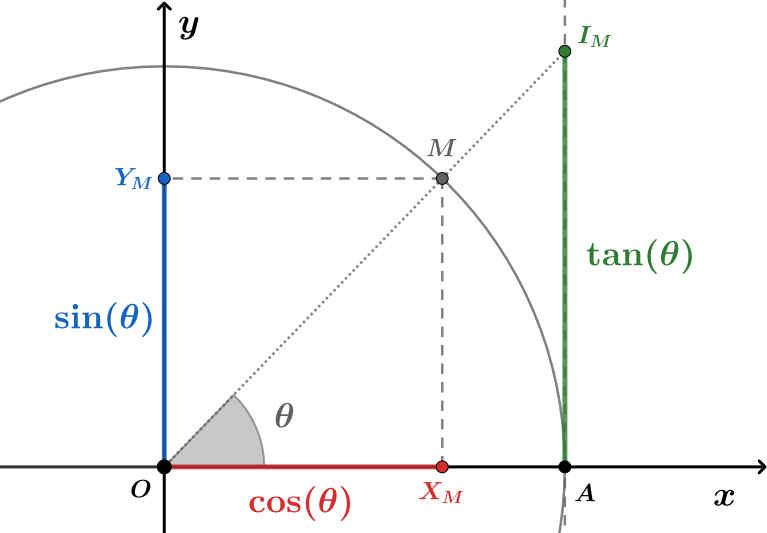
\includegraphics[width=8cm]{Image/Cercle Trigo/Cercle_trigo_lien_avec_fct_trigo.png}
			\end{center}

			\vspace{-0.5cm}
			
			\subsubsection{Retrouver le sinus et le cosinus de $\theta$}

			À l'aide des définitions des fonctions sinus et cosinus,
			il facile de calculer les longueurs des côtés de ce triangle :

			\begin{tabular}{ll}
				$\text{Cathète Adjacente} = \cos(\theta) \times \text{Hypoténuse}$ & $\Longrightarrow$ Longueur de $[OX_M]$ = $\cos(\theta) \times 1$\\
				$\text{Cathète Opposée} = \sin(\theta) \times \text{Hypoténuse}$   & $\Longrightarrow$ Longueur de $[MX_M]$ = $\sin(\theta) \times 1$\\
			\end{tabular}
			
			\medbreak

			De plus, il est possible de tracer un second triangle rectangle $OMY_M$ ayant pour hypoténuse le rayon du cercle.
			Les longueurs des côtés de ce nouveau triangle sont les mêmes que celles du triangle $OMX_M$.

			Ainsi on peut en conclure que,
			les coordonnées cartésiennes du point $M$ sont $(\cos(\theta), \sin(\theta))$.
			Réciproquement, pour chaque point du cercle,
			il est possible d'obtenir le sinus et le cosinus de l'angle correspondant,
			en projetant ce point sur l'axe des abscisses et sur celui des ordonnées.\footnote{
				J'utilise un moyen mnémotechnique pour retenir quel axe est celui où l'on retrouve le sinus de l'angle.
				L'abréviation de sinus c'est sin, ce qui correspond au début du mot "singe", 
				les singes montent dans les arbres, par conséquent l'axe des sinus est l'axe verticale de notre repère.
			}

			\subsubsection{Retrouver la tangente de $\theta$}
			De plus, on peut aussi retrouver graphiquement la tangente :
			\begin{itemize}
				\item [•] Prenez la droite tangente (géométriquement) au cercle, étant perpendiculaire à l'axe des abscisse positives et passant par $A$.
				\item [•] Prolongez le rayon terminant l'angle $\theta$. Cette demi-droite coupe la tangente géométrique en un point $I_M$.
				\item [•] La longueur de $[AI_M] = \tan(\theta)$.
			\end{itemize}

			\vspace{-0.25cm}

			\paragraph*{Démonstration :} Nous savons que $OA = 1$, que $OX_M = \cos(\theta)$ et que $X_MM = \sin(\theta)$.
			De plus, nous pouvons remarquer que les triangles $OMX_M$ et $OI_MA$ sont semblables, car ils sont équiangles.

			Grâce à cette propriété, nous pouvons utiliser le théorèmes de \textsc{Thalès}, nous indiquant que $\frac{OX_M}{OA} = \frac{X_MM}{AI_M}$.
			En réarrangeant cette équation, on obtient : 
				$${AI_M} = \frac{X_MM \times OA}{OX_M} = \frac{\sin(\theta) \times 1}{\cos(\theta)} = \frac{\sin(\theta)}{\cos(\theta)}$$

			Et comme présenté précédemment (à la page n°\pageref{lien_fct_trigo}), 
			il existe un lien entre les trois fonctions trigonométriques élémentaires, 
			à l'aide de ce lien, on démontre enfin que : 
				$${AI_M} = \tan(\theta)$$

\newpage

		\subsection{Périodicité et mesure principale}

			En tournant autour du cercle trigonométrique,
			il est possible d'obtenir un angle mesurant n'importe quel réel.
			
			Ainsi, sur n'importe quel point du cercle,
			peut être représenté plusieurs angles ayant des mesures
			différant d'un certain nombre de tours du cercle.

			Comme un tour complet du cercle correspond à un angle de $2 \pi$ radians,
			pour un angle $\theta$ donné,
			les angles $\theta + 2 \pi \times k$ (avec $k \in \mathbb{Z}$)
			tombent sur le même point du cercle.

			\medbreak

			Comme nous l'avons vu, la mesure d'un angle en radians est la longueur de 
			l'arc de cercle intercepté par cet angle,
			ainsi les propriétés des fonctions trigonométriques 
			seront nécessairement \emph{$2\pi$-périodiques},
			c'est-à-dire qu'elles se répètent tous les $2 \pi$ radians.

			Par conséquent, nous allons nous intéresser uniquement à la \emph{mesure principale} 
			des angles représentés sur le cercle.
			La mesure principale d'un angle donné est la mesure
			d'un angle compris entre $-\pi$ rad et $\pi$ rad,
			tombant sur le même point du cercle que l'angle initial.

			De plus comme $-\pi$ rad et $\pi$ rad sont les mêmes points du cercle,
			on dira que la mesure principale de $-\pi$ rad est $\pi$ rad.
			
			Ainsi, pour un angle $\theta$ donné,
			sa mesure principale est définie comme étant comprise dans l'intervale $]-\pi, \pi]$.

\newpage

	\section{Propriété des fonctions trigonométriques}

		Les fonctions sinus, cosinus et tangente sont les trois fonctions trigonométriques
		les plus utilisées en mathématique. Ce sont les valeurs prisent par ces fonctions
		qui sont représentées dans la table.

		\subsection{Valeurs remarquables}

			Voici un tableau regroupant les valeurs remarquables des fonctions sinus, cosinus et tangente :

			\begin{center}
				%\renewcommand{\arraystretch}{1.75}
				\setcellgapes{1.5mm}
				\makegapedcells
				\begin{tabular}{|l||c||c|c|c||c||c|c|c||c|}
					\hline
					Angle $\theta$ & $0$ & {\large $\frac{\pi}{6}$} & {\large $\frac{\pi}{4}$} & {\large $\frac{\pi}{3}$} & {\large $\frac{\pi}{2}$} & {\large $\frac{2\pi}{3}$} & {\large $\frac{3\pi}{4}$} & {\large $\frac{5\pi}{6}$} & $\pi$\\
					\hline
					\hline
					$\sin(\theta)$ & $0$ & {\large $\frac{1}{2}$} & {\large $\frac{\sqrt{2}}{2}$} & {\large $\frac{\sqrt{3}}{2}$} & $1$ & {\large $\frac{\sqrt{3}}{2}$} & {\large $\frac{\sqrt{2}}{2}$} & {\large $\frac{1}{2}$} & $0$ \\
					\hline
					$\cos(\theta)$ & $1$ & {\large $\frac{\sqrt{3}}{2}$} & {\large $\frac{\sqrt{2}}{2}$} & {\large $\frac{1}{2}$} & $0$ & {\large $-\frac{1}{2}$} & {\large $-\frac{\sqrt{2}}{2}$} & {\large $-\frac{\sqrt{3}}{2}$} & $-1$ \\
					\hline
					$\tan(\theta)$ & $0$ & {\large $\frac{\sqrt{3}}{3}$} & $1$ & $\sqrt{3}$ & \textcolor{Red}{\LARGE {$\times$}} & $-\sqrt{3}$ & $-1$ & {\large $-\frac{\sqrt{3}}{3}$ } & $0$ \\
					\hline
				\end{tabular}
			\end{center}

			Comme ces fonctions sont $2\pi$-périodiques,
			les valeurs remarquables de ces fonctions se répètent tous les $2\pi$ radians.
			C'est pourquoi, dans ce tableau, 
			les valeurs remarquables sont données pour les angles compris entre $0$ et $\pi$ radians.

			\vfill

			Il est possible de retrouver facilement ces valeurs 
			à l'aide du cercle trigonométrique, en se souvenant du
			schéma suivant :
			
			\begin{multicols}{2}

				\begin{center}
					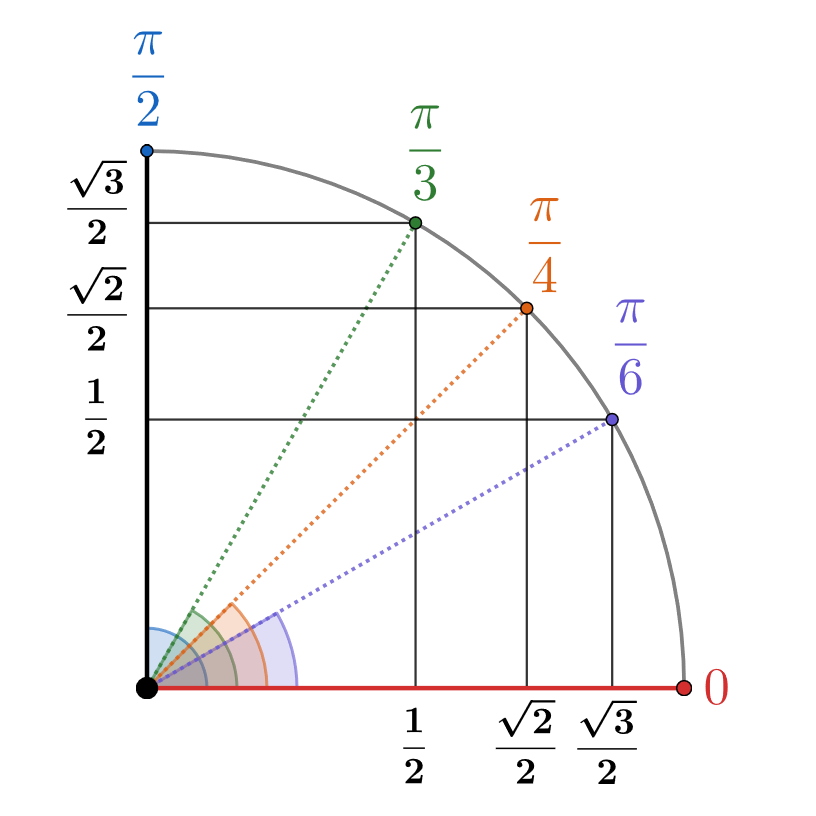
\includegraphics[height=7.8cm]{Image/Cercle Trigo/cercle_trigo_valeur_remarquable.PNG}
				\end{center}

				Ce schéma représente une portion du cercle trigonométrique,
				dont les points ont une abscisse et une ordonnée positive.
				C'est la portion la plus utile du cercle trigonométrique.

				\paragraph*{Comment tracer ce schéma}

				Pour tracer les 6 segments nous indiquant les valeurs de sinus et cosinus,
				des angles de $\frac{\pi}{6}$, $\frac{\pi}{4}$ et $\frac{\pi}{3}$,
				il faut tracer dans un premier les deux segments à l'abscisse et l'ordonnée égale à $\frac{1}{2}$.

				Ces deux premiers segments croisent le cercle en deux points,
				le premier point est celui de l'angle $\frac{\pi}{6}$,
				et le second est celui de l'angle $\frac{\pi}{3}$.
				Maintenant que nous avons ces deux points,
				il est possible de tracer les deux segments à l'abscisse et l'ordonnée égale à $\frac{\sqrt{3}}{2}$.

				\phantom{dhdgdj}

				\phantom{dhdgdj}

			\end{multicols}

			Pour obtenir les deux derniers segments, 
			nous allons d'abords tracer le rayon passant par le point de d'intersection
			des deux premiers segments.
			Ce rayon coupe le cercle en un point,
			qui est celui correspondant à l'angle $\frac{\pi}{4}$.
			Et enfin, nous pouvons à l'aide de ce point,
			tracer les deux derniers segments.
			
			\paragraph*{Angles ayant des valeurs de sinus et cosinus exactes}
			\phantom{r}

			On peut remarquer que les angles opposés à ceux du tableau ont aussi 
			des valeurs de sinus et cosinus exactes.
			Leur cosinus restera le même, mais leur sinus sera négatif. 
			
			Il existe d'autres angles ayant des valeurs de sinus, de cosinus et de tangente exactes,
			certaines de ces valeurs sont présentés en Annexe, à la page \pageref{valeur_remarquable_trigo}.

		\subsection{Étude de fonction}
			\subsubsection{Définition de ces fonctions}
				\paragraph*{Définition}
					\phantom{r}

					Les fonction sinus et cosinus associe à tout réel $x$, le réel $\sin(x)$ et $\cos(x)$.
					La fonction tangente associe à la majorité des réels $x$, le réel $\tan(x)$.				
					
					Dans notre cas, $x$ est un angle orienté suivant la convention du cercle trigonométrique, présenté plus tôt.
					De plus, nous considérons que $x$ est exprimé en \emph{radians}.

				\paragraph*{Domaine de définition et ensemble d'arrivée}
					\phantom{r}

					Pour les fonctions sinus et cosinus :
					\begin{itemize}
						\item [•] Leur domaine de définition est $\mathbb{R}$.
						\item [•] Leur ensemble d'arrivée est l'intervalle $[-1~;~1]$.
					\end{itemize}

					\vspace{2mm}

					Pour la fonction tangente :
					\begin{itemize}
						\item [•] Son domaine de définition est $\mathbb{R} \setminus \{\left. k\pi+\frac{\pi}{2} ~ \right| ~ k \in \mathbb{Z}\}$.
						\item [•] Son ensemble d'arrivée est $\mathbb{R}$.
					\end{itemize}

			\subsubsection{Propriétés de ces fonctions}
				\paragraph*{Périodicité}
					\phantom{r}

					Les fonctions sinus, cosinus et tangente sont $2\pi$-périodiques.
					C'est à dire que, tout les $2\pi$ radians, ces fonctions se répètent.
					
					Ainsi : $\forall x \in \mathbb{R}$, $\sin(x) = \sin(x + 2\pi)$, $\cos(x) = \cos(x + 2\pi)$ et $\tan(x) = \tan(x + 2\pi)$
				\paragraph*{Parité}
					\phantom{r}

					La fonction sinus est impaire, la fonction cosinus est paire\footnote{
						Une fonction $f$ est impaire, si $\forall x \in \mathbb{R}, f(x) = -f(x)$.
						Une fonction $f$ est paire, si $\forall x \in \mathbb{R}, f(x) = f(-x)$.}.
					
					La fonction tangente est impaire sur l'intervale $\left] -\frac{\pi}{2}~;~\frac{\pi}{2} \right[$, 
					elle n'est en revanche ni paire, ni impaire sur $\mathbb{R}$.

				\paragraph*{Variation sur $\left] -\pi ~;~ \pi\right]$}
					\phantom{r}
					
					Comme ces trois fonctions sont $2\pi$-périodiques,
					nous pouvons nous intéresser uniquement à leur variation sur l'intervale $\left] -\pi ~;~ \pi \right]$ :

					\vspace{3mm}
					\noindent{
					\begin{tikzpicture}
						\tkzTabInit{$x$ / 0.75 , $\sin(x)$ / 1.25, $\cos(x)$ / 1.25, $\tan(x)$ / 1.25}{$-\pi$, $-\frac{\pi}{2}$, $0$, $\frac{\pi}{2}$, $\pi$}
						\tkzTabVar{+/ $0$, -/ $-1$, R/, +/ $1$, -/ $0$}
						\tkzTabIma{2}{4}{3}{$0$}
						\tkzTabVar{-/ $-1$, R/, +/ $1$, R/, -/ $-1$}
						\tkzTabIma{1}{3}{2}{$0$}
						\tkzTabIma{3}{5}{4}{$0$}
						\tkzTabVar{-/$0$, +D-/ $+\infty$ / $-\infty$, R/,+D-/ $+\infty$ / $-\infty$, +/$0$}
						\tkzTabIma{2}{4}{3}{$0$}
					\end{tikzpicture}
					}

				\vspace{-5mm}
				
				\paragraph*{Dérivée}
					\phantom{r}

					\begin{tabular}{lclcl}
						$\sin'(u(x))$ & $=$ & $\phantom{-}u'(x) \times \cos(u(x))$ & & \phantom{\large{$\frac{u'(x)}{\cos^2(u(x))}$}}\\
						$\cos'(u(x))$ & $=$ & $-u'(x) \times \sin(u(x))$ && \phantom{\large{$\frac{u'(x)}{\cos^2(u(x))}$}}\\
						$\tan'(u(x))$ & $=$ & $\phantom{-}u'(x) \times (1 + \tan^2(u(x)))$ & $ = $ & \large{$\frac{u'(x)}{\cos^2(u(x))}$} \\
					\end{tabular}

					\vfill
					\vspace{5mm}

				\noindent{\textit{Démonstration de ces propriétés en Annexe, à la page \pageref{demo_propriete_trigo_1}.}}

\newpage
		\subsubsection{Représentation graphique}
			\vspace*{-0.25cm}
			\begin{center}
				\makebox[\textwidth][c]{
					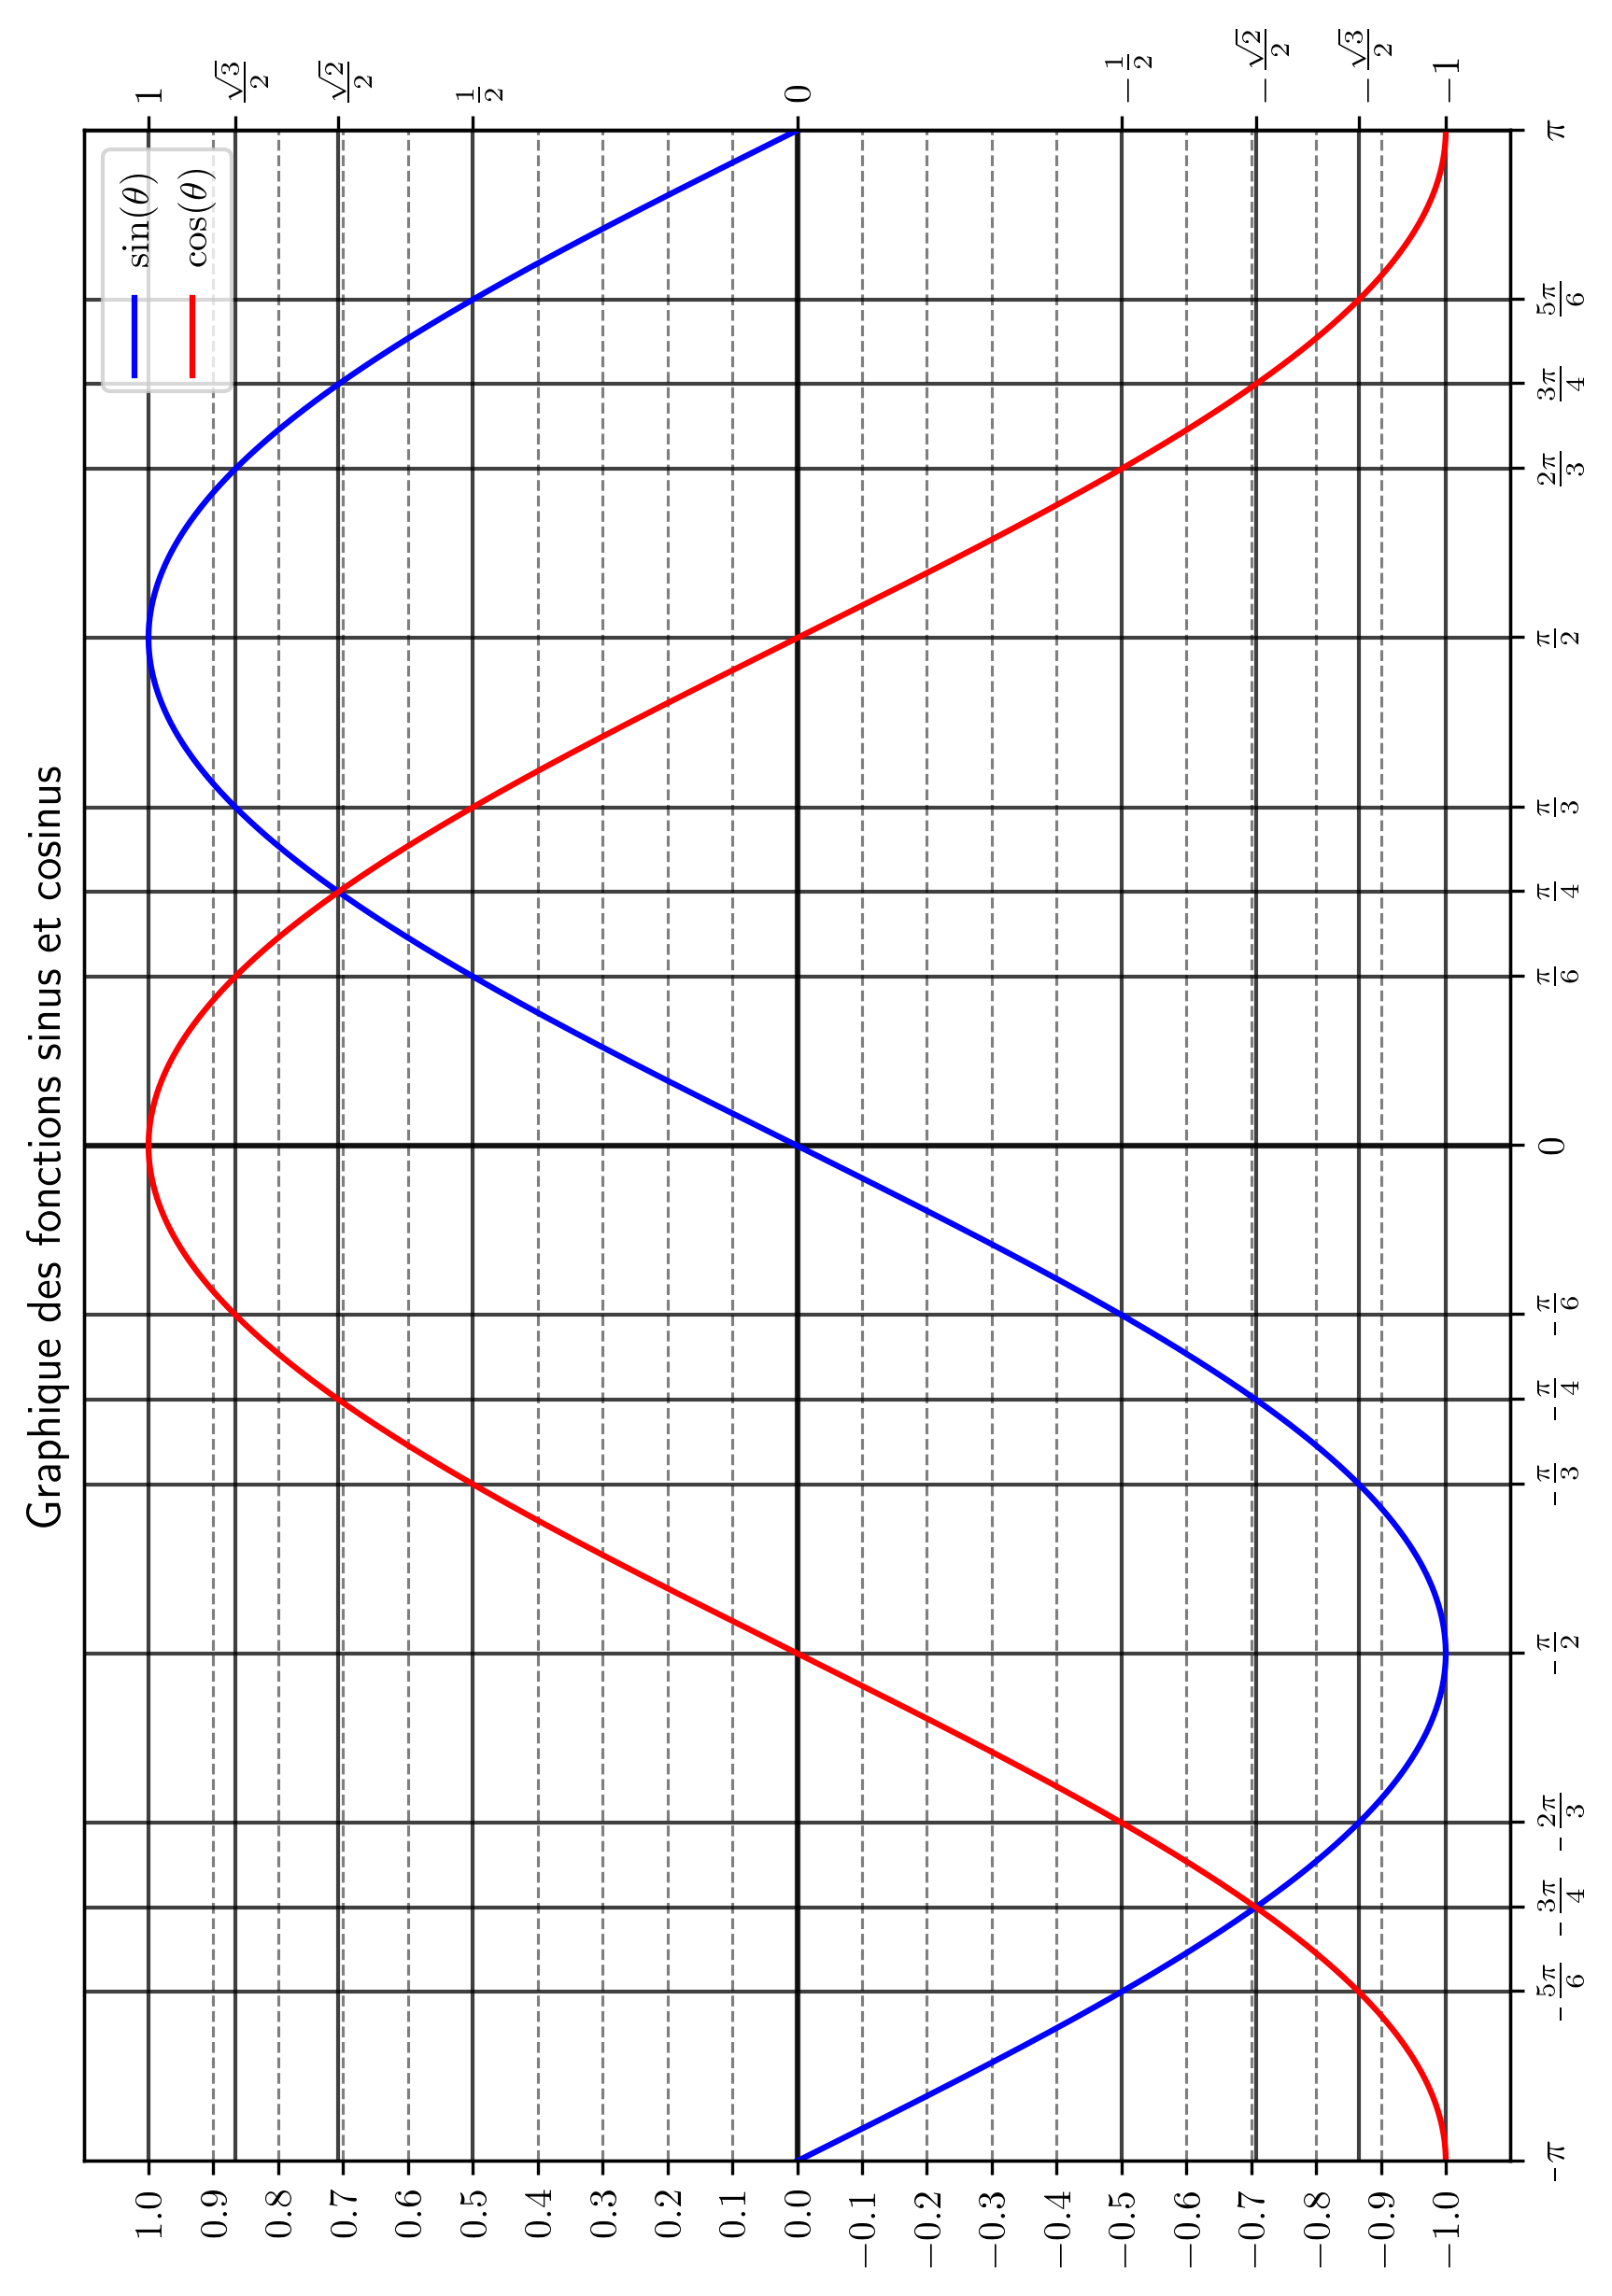
\includegraphics[height=24cm]{Graphs fonctions/sinus_cosinus_modifie.png}
				}
			\end{center}

\newpage

			\vspace*{-0.25cm}
			\begin{center}
				\makebox[\textwidth][c]{
					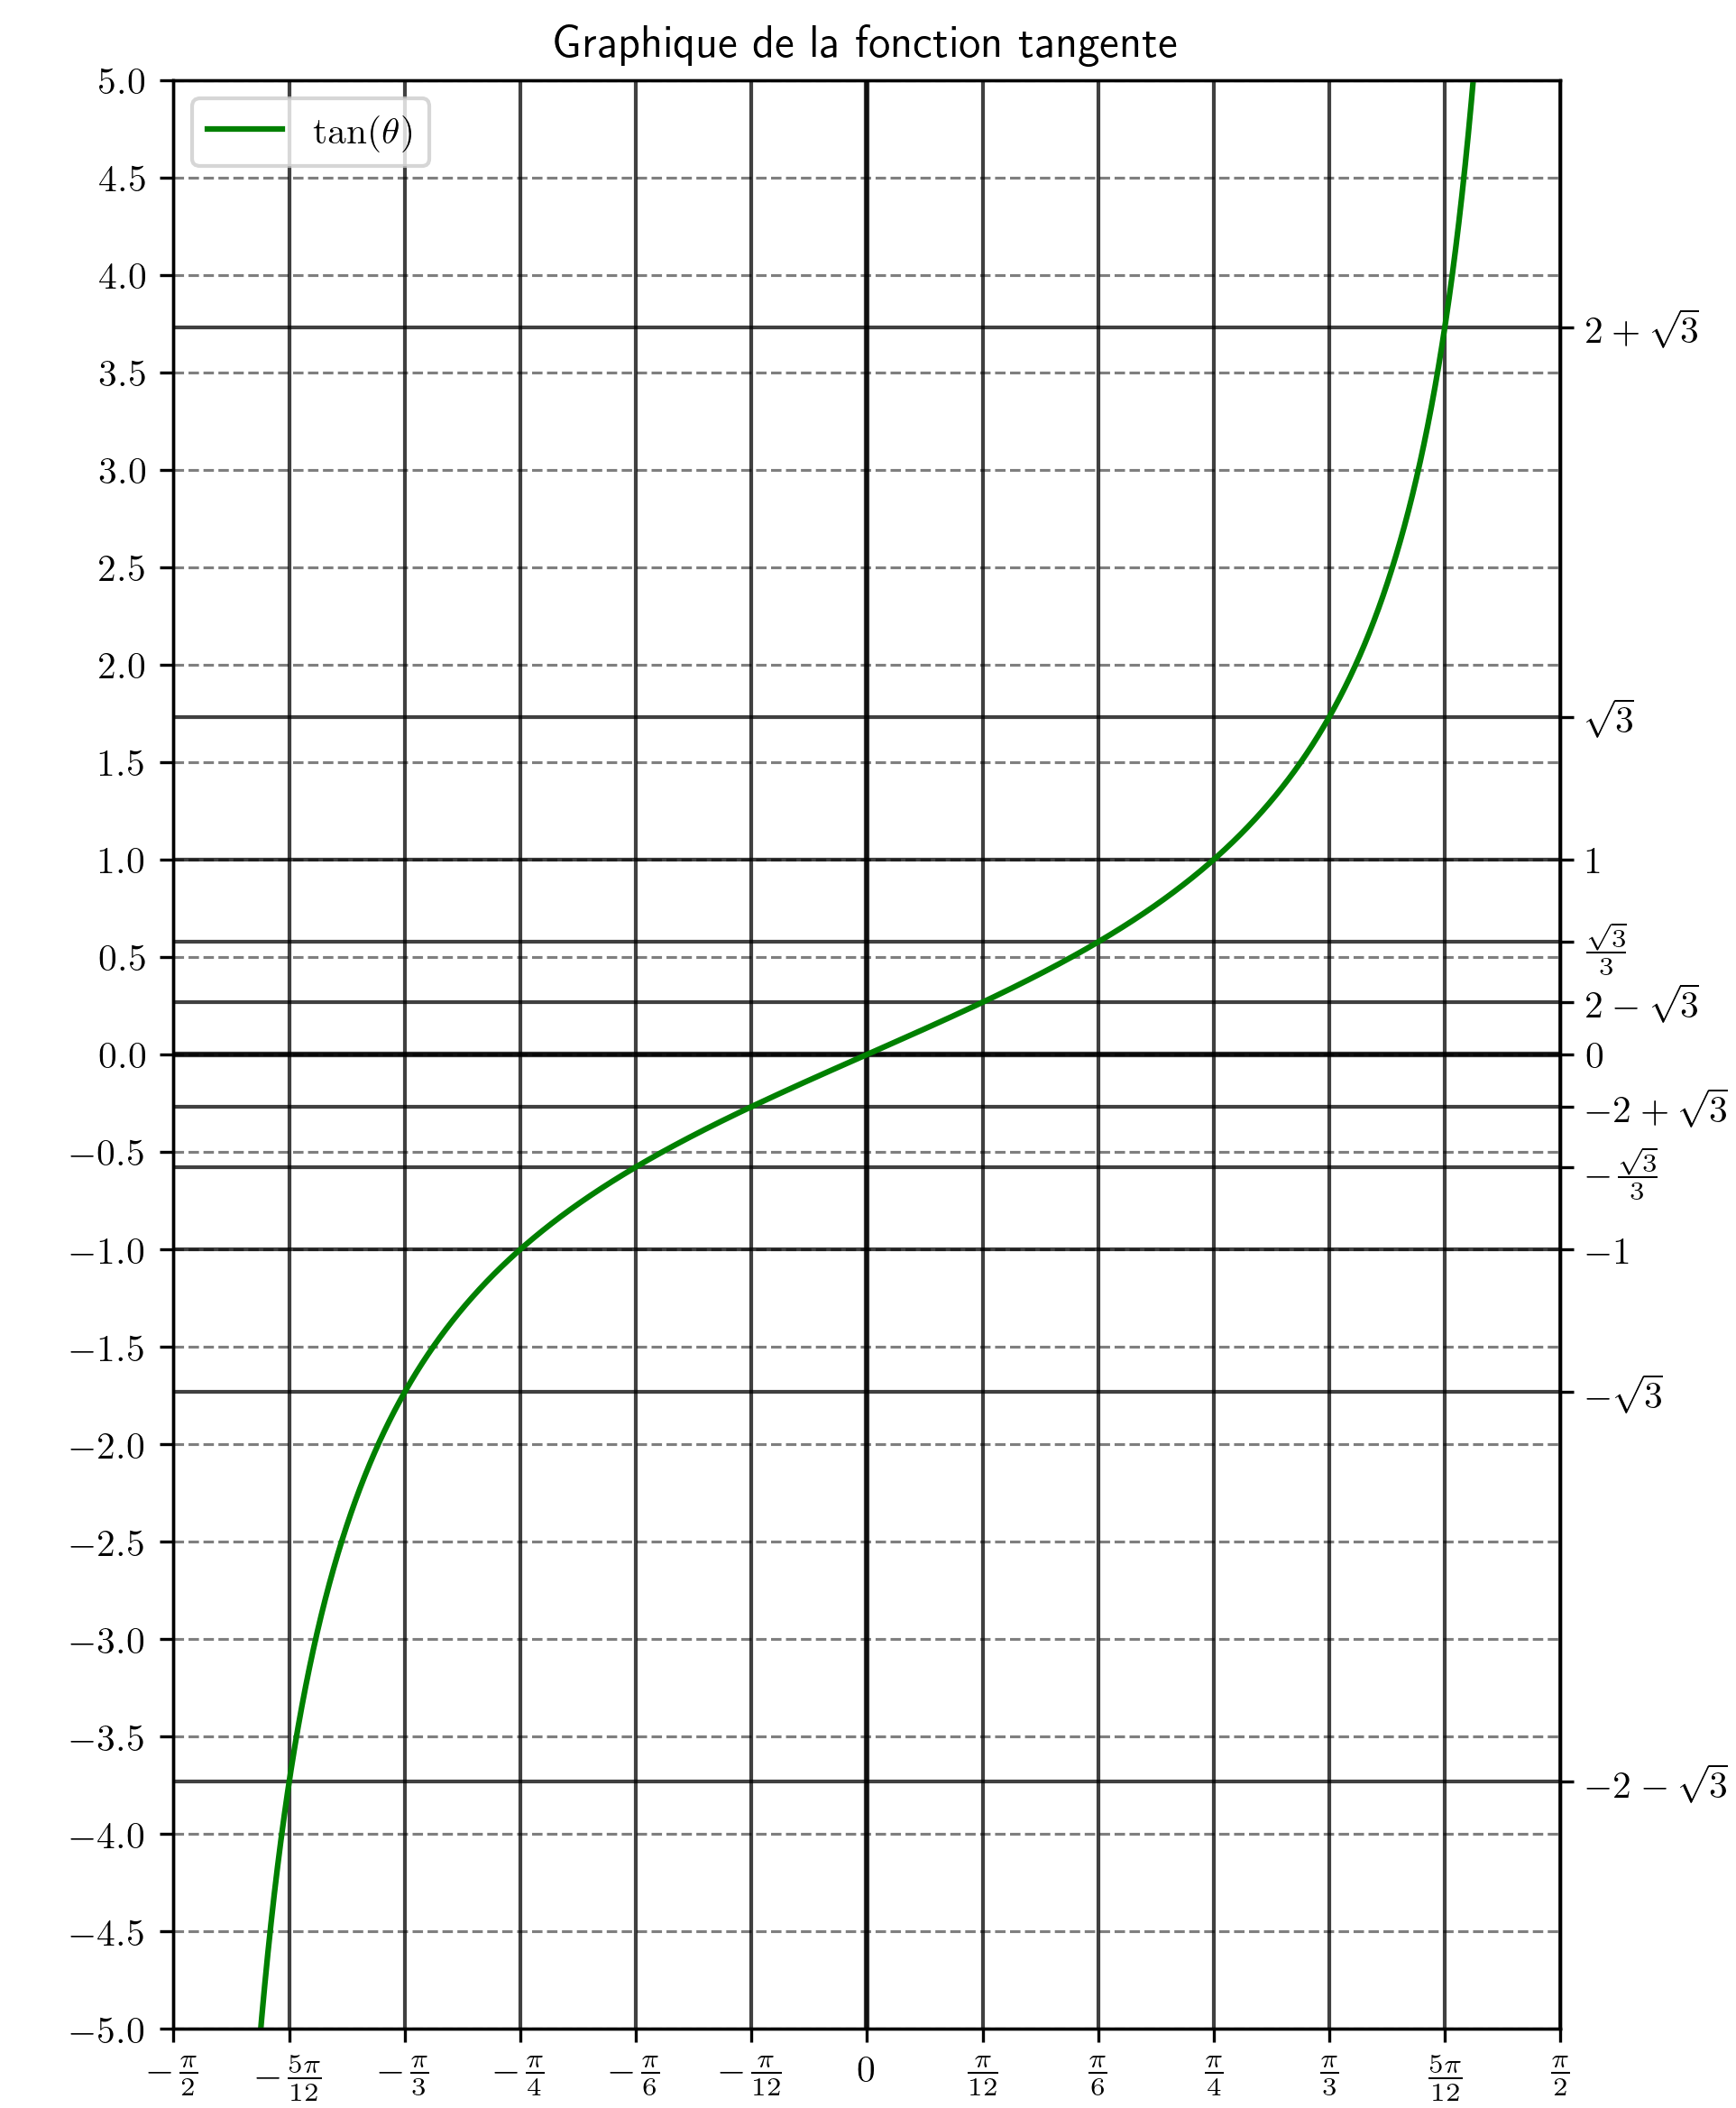
\includegraphics[height=23.25cm]{Graphs fonctions/tangente_modifie.png}
				}
			\end{center}

\newpage

	\section{Fonctions trigonométriques inverses}
		
		\subsection*{Définition}

			Les fonctions trigonométriques inverses sont les fonctions réciproques des fonctions trigonométriques.
			Ce sont les fonctions \emph{arcsinus}, \emph{arccosinus} et \emph{arctangente}. Elles sont notées $\arcsin$, $\arccos$ et $\arctan$.

			Elle nous permettent de retrouver quel angle correspond a une certaine valeur de sinus, de cosinus ou de tangente.
			Ou encore, elles nous permettent de retrouver la longueur de l'\textit{arc} du cercle trigonométrique\footnote{
				Pour rappel, la longueur d'un arc de cercle délimité par un angle $\theta$, est égale à $\theta$, si :
				\begin{itemize}
					\item [•] Le rayon du cercle est égal à 1, ce qui est le cas dans le cercle trigonométrique.
					\item [•] L'angle est exprimé en radians, par définition de cette unité.
				\end{itemize}
				\vspace*{-0.25cm}
				} donnant ce sinus ce cosinus ou cette tangente. C'est pour cette raison que  l'on retrouve le préfixe \textit{arc} dans leur nom.

			\subsubsection*{Fonctions réciproques}

			Ce sont des fonctions réciproques, comme pour la fonction racine carrée et la fonction carrée.
			Ainsi, pour tout $x$ dans leur ensemble d'arrivée, on a : $f^{-1}(f(x)) = x$.
			C'est pour cela que ces fonctions sont parfois notées $\sin^{-1}$, $\cos^{-1}$ et $\tan^{-1}$.

			Mais comme pour la fonction carré, la réciproque n'est vrai que dans certaines conditions\footnote{$\forall x \in \mathbb{R}^{+}, x = \sqrt{x^2} = \sqrt{x}^2$.
			
			~~Mais dans $\mathbb{R}$ : $\forall x \in \mathbb{R}, \sqrt{x^2} = |x|$ et $\sqrt{x}^2$ n'est pas toujours définie (car $\forall x \in \mathbb{R}^-, \sqrt{x}$ n'est pas définie)}.
			Dans le cas des fonctions trigonométriques, ces fonctions étant périodiques,
			nous devons sélectionner un intervalle de définition, qui servira d'ensemble d'arrivée de chacune de ces fonctions.
			
			\subsection*{Domaine de définition et ensemble d'arrivée}

				\begin{center}
					\setcellgapes{1.5mm}
					\makegapedcells
					\begin{tabular}{|c|c|c|}
						\hline
						\textbf{Fonction} & \textbf{Domaine de définition} & \textbf{Ensemble d'arrivée} \\
						\hline
						$\arcsin$ & $[-1~;~1]$ & $[-\frac{\pi}{2}~;~\frac{\pi}{2}]$ \\
						\hline
						$\arccos$ & $[-1~;~1]$ & $[0~;~\pi]$\\
						\hline
						$\arctan$ & $\mathbb{R}$ & $\left]-\frac{\pi}{2}~;~\frac{\pi}{2}\right[$\\
						\hline
					\end{tabular}
				\end{center}
			
			\subsubsection*{Variation sur leur domaine de définition respectif}

				\begin{center}
					\begin{tikzpicture}
						\tkzTabInit{$x$ / 0.75 , $\arcsin(x)$ / 1.25 , $\arccos(x)$ / 1.25}{$-1$, $0$, $1$}
						\tkzTabVar{-/ $-\frac{\pi}{2}$, R/, +/ $+\frac{\pi}{2}$}
						\tkzTabIma{1}{3}{2}{$0$}
						\tkzTabVar{+/ $\pi$, R/, -/ $0$}
						\tkzTabIma{1}{3}{2}{$\frac{\pi}{2}$}
					\end{tikzpicture}

					\vspace{0.2cm}
					
					\begin{tikzpicture}
						\tkzTabInit{$x$ / 0.75 , $\arctan(x)$ / 1.25}{$-\infty$, $0$, $+\infty$}
						\tkzTabVar{-/ $-\frac{\pi}{2}$,R/, +/ $+\frac{\pi}{2}$}
						\tkzTabIma{1}{3}{2}{$0$}
					\end{tikzpicture}
				\end{center}
			
			\vspace*{-0.5cm}

			\subsubsection*{Dérivée}

				\begin{tabular}{lclcl}
					$\arcsin'(u(x))$ & $=$ & $\phantom{-}\frac{u'(x)}{\sqrt{1 - u(x)^2}}$ & & \\
					$\arccos'(u(x))$ & $=$ & $-\frac{u'(x)}{\sqrt{1 - u(x)^2}}$ & & \\
					$\arctan'(u(x))$ & $=$ & $\phantom{-}\frac{u'(x)}{1 + u(x)^2}$ & $ = $ & $\frac{u'(x)}{\cos^2(u(x))}$ \\
				\end{tabular}

\newpage
			\vspace*{-1cm}
			\begin{center}
				\makebox[\textwidth][c]{
					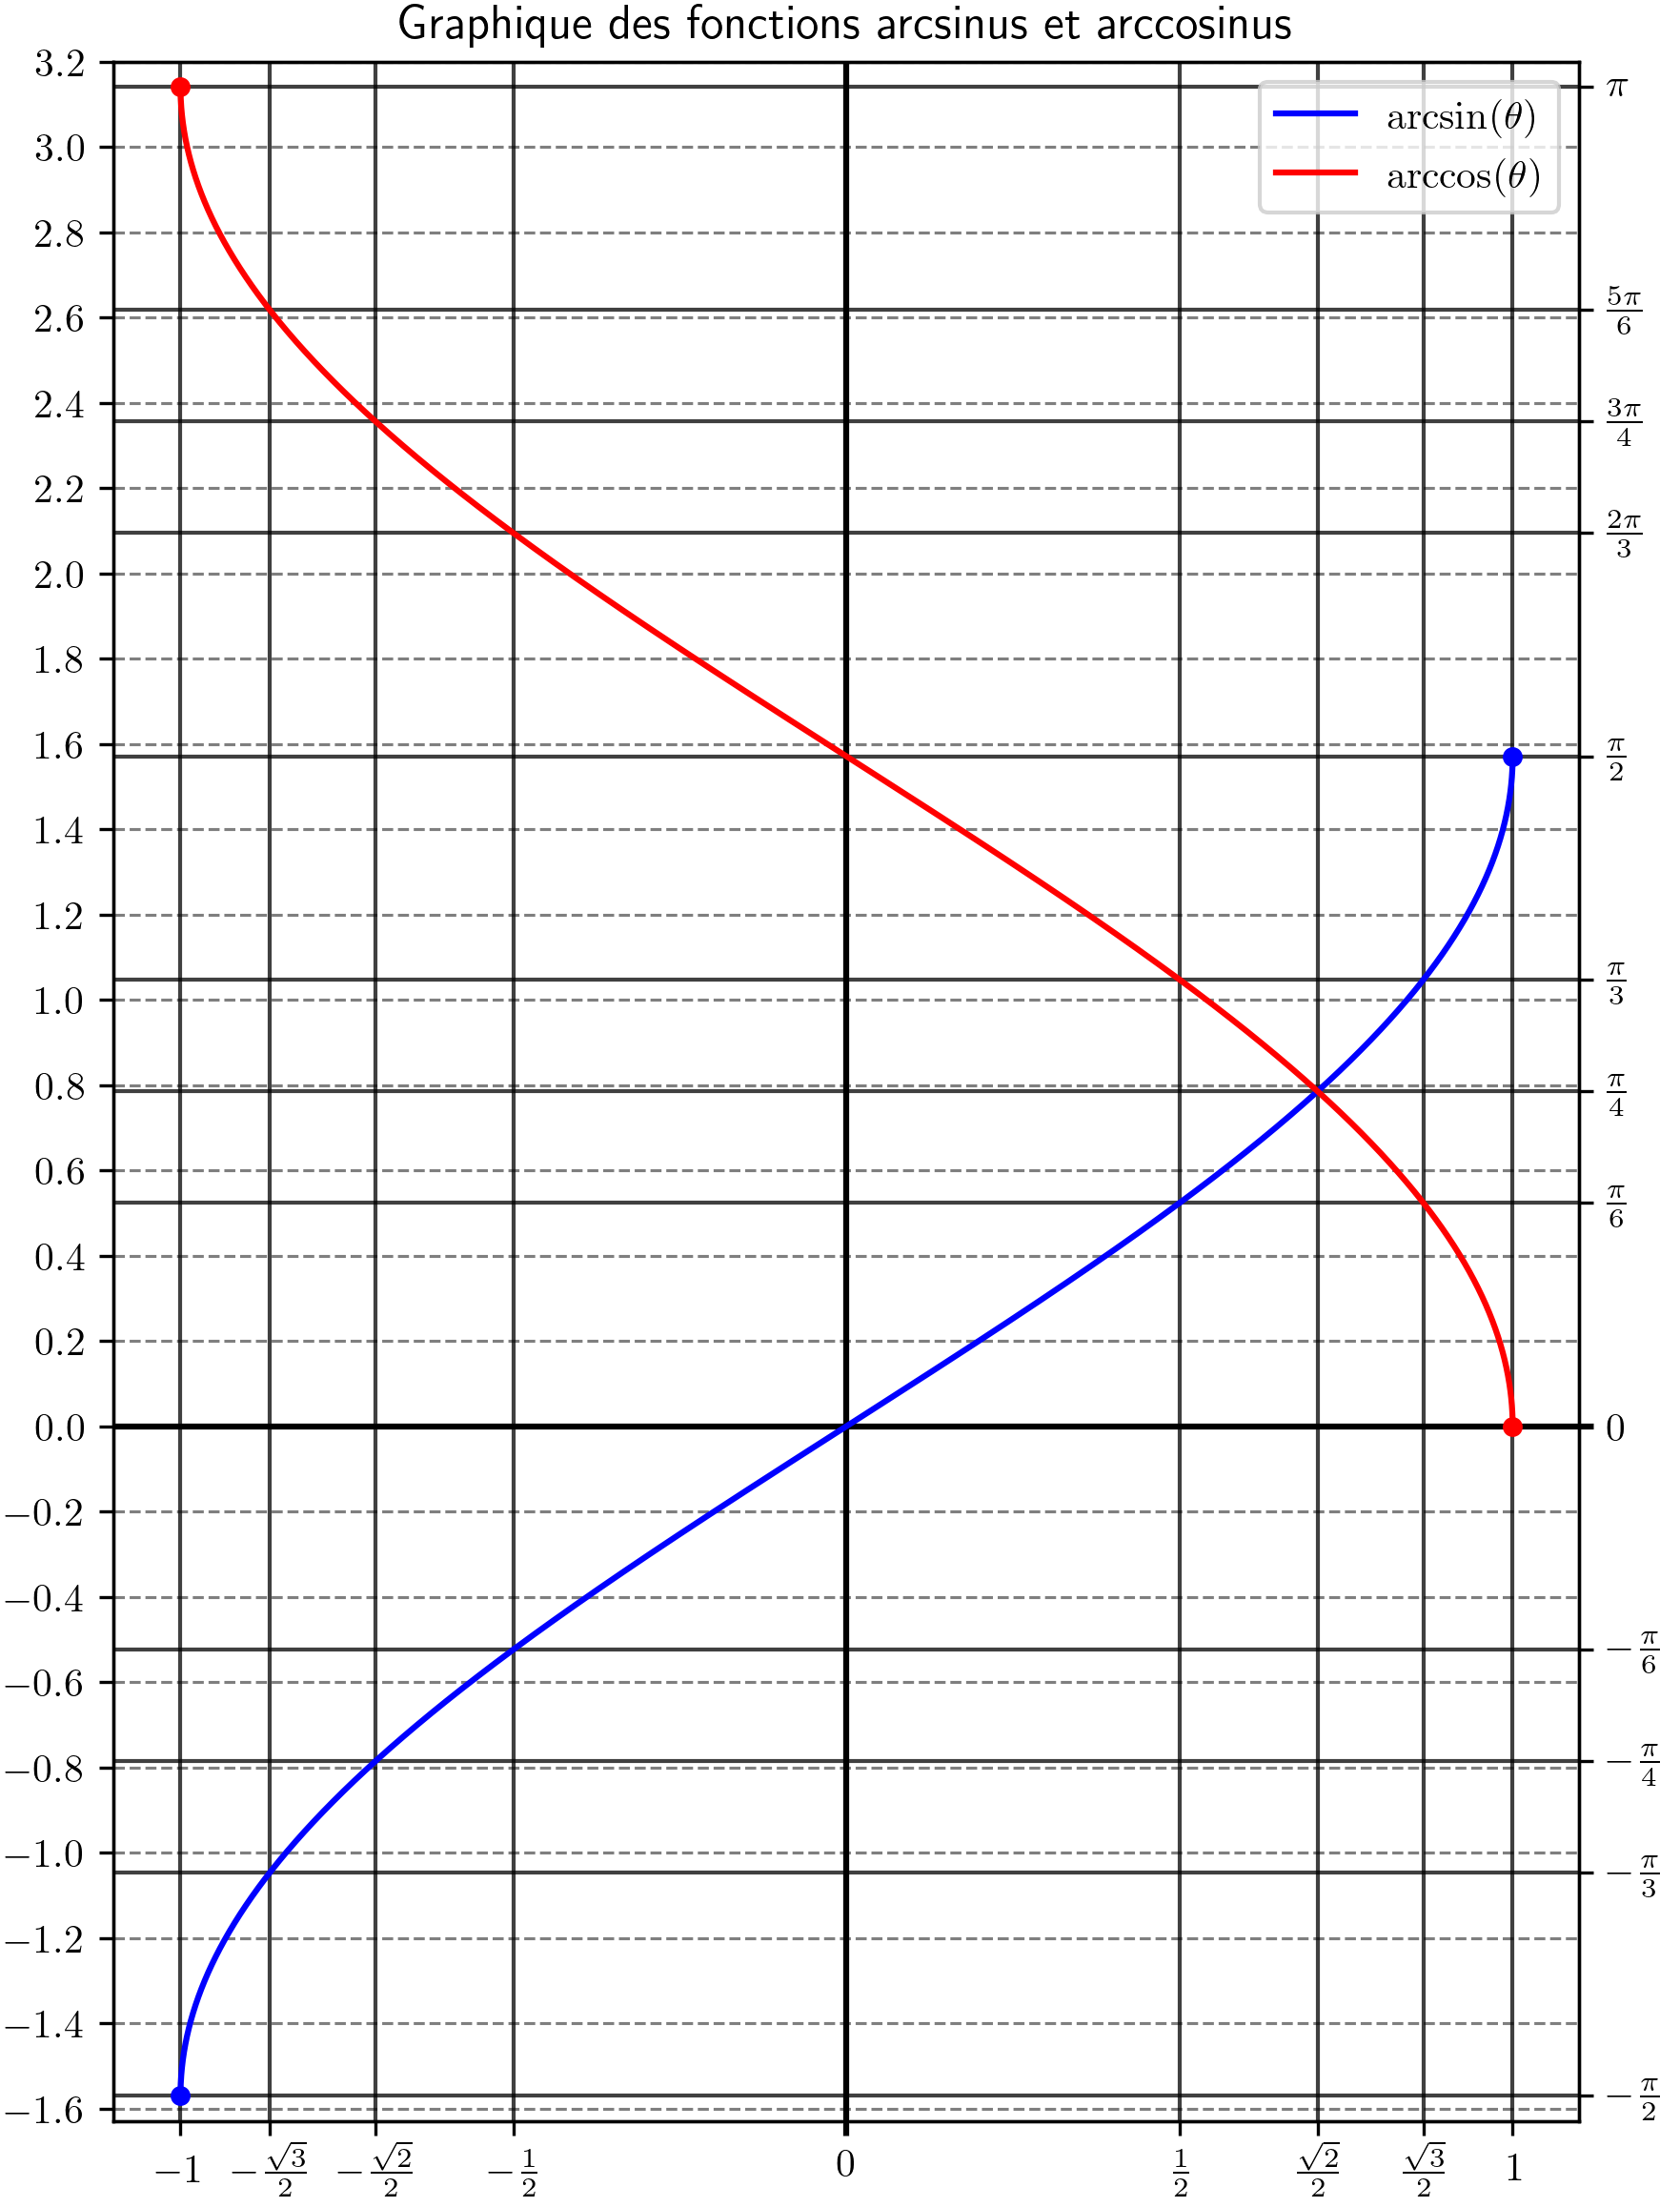
\includegraphics[height=24cm]{Graphs fonctions/arcsinus_arccosinus_modifie.png}
				}
			\end{center}

\newpage
			\vspace*{-1cm}
			\begin{center}
				\makebox[\textwidth][c]{
					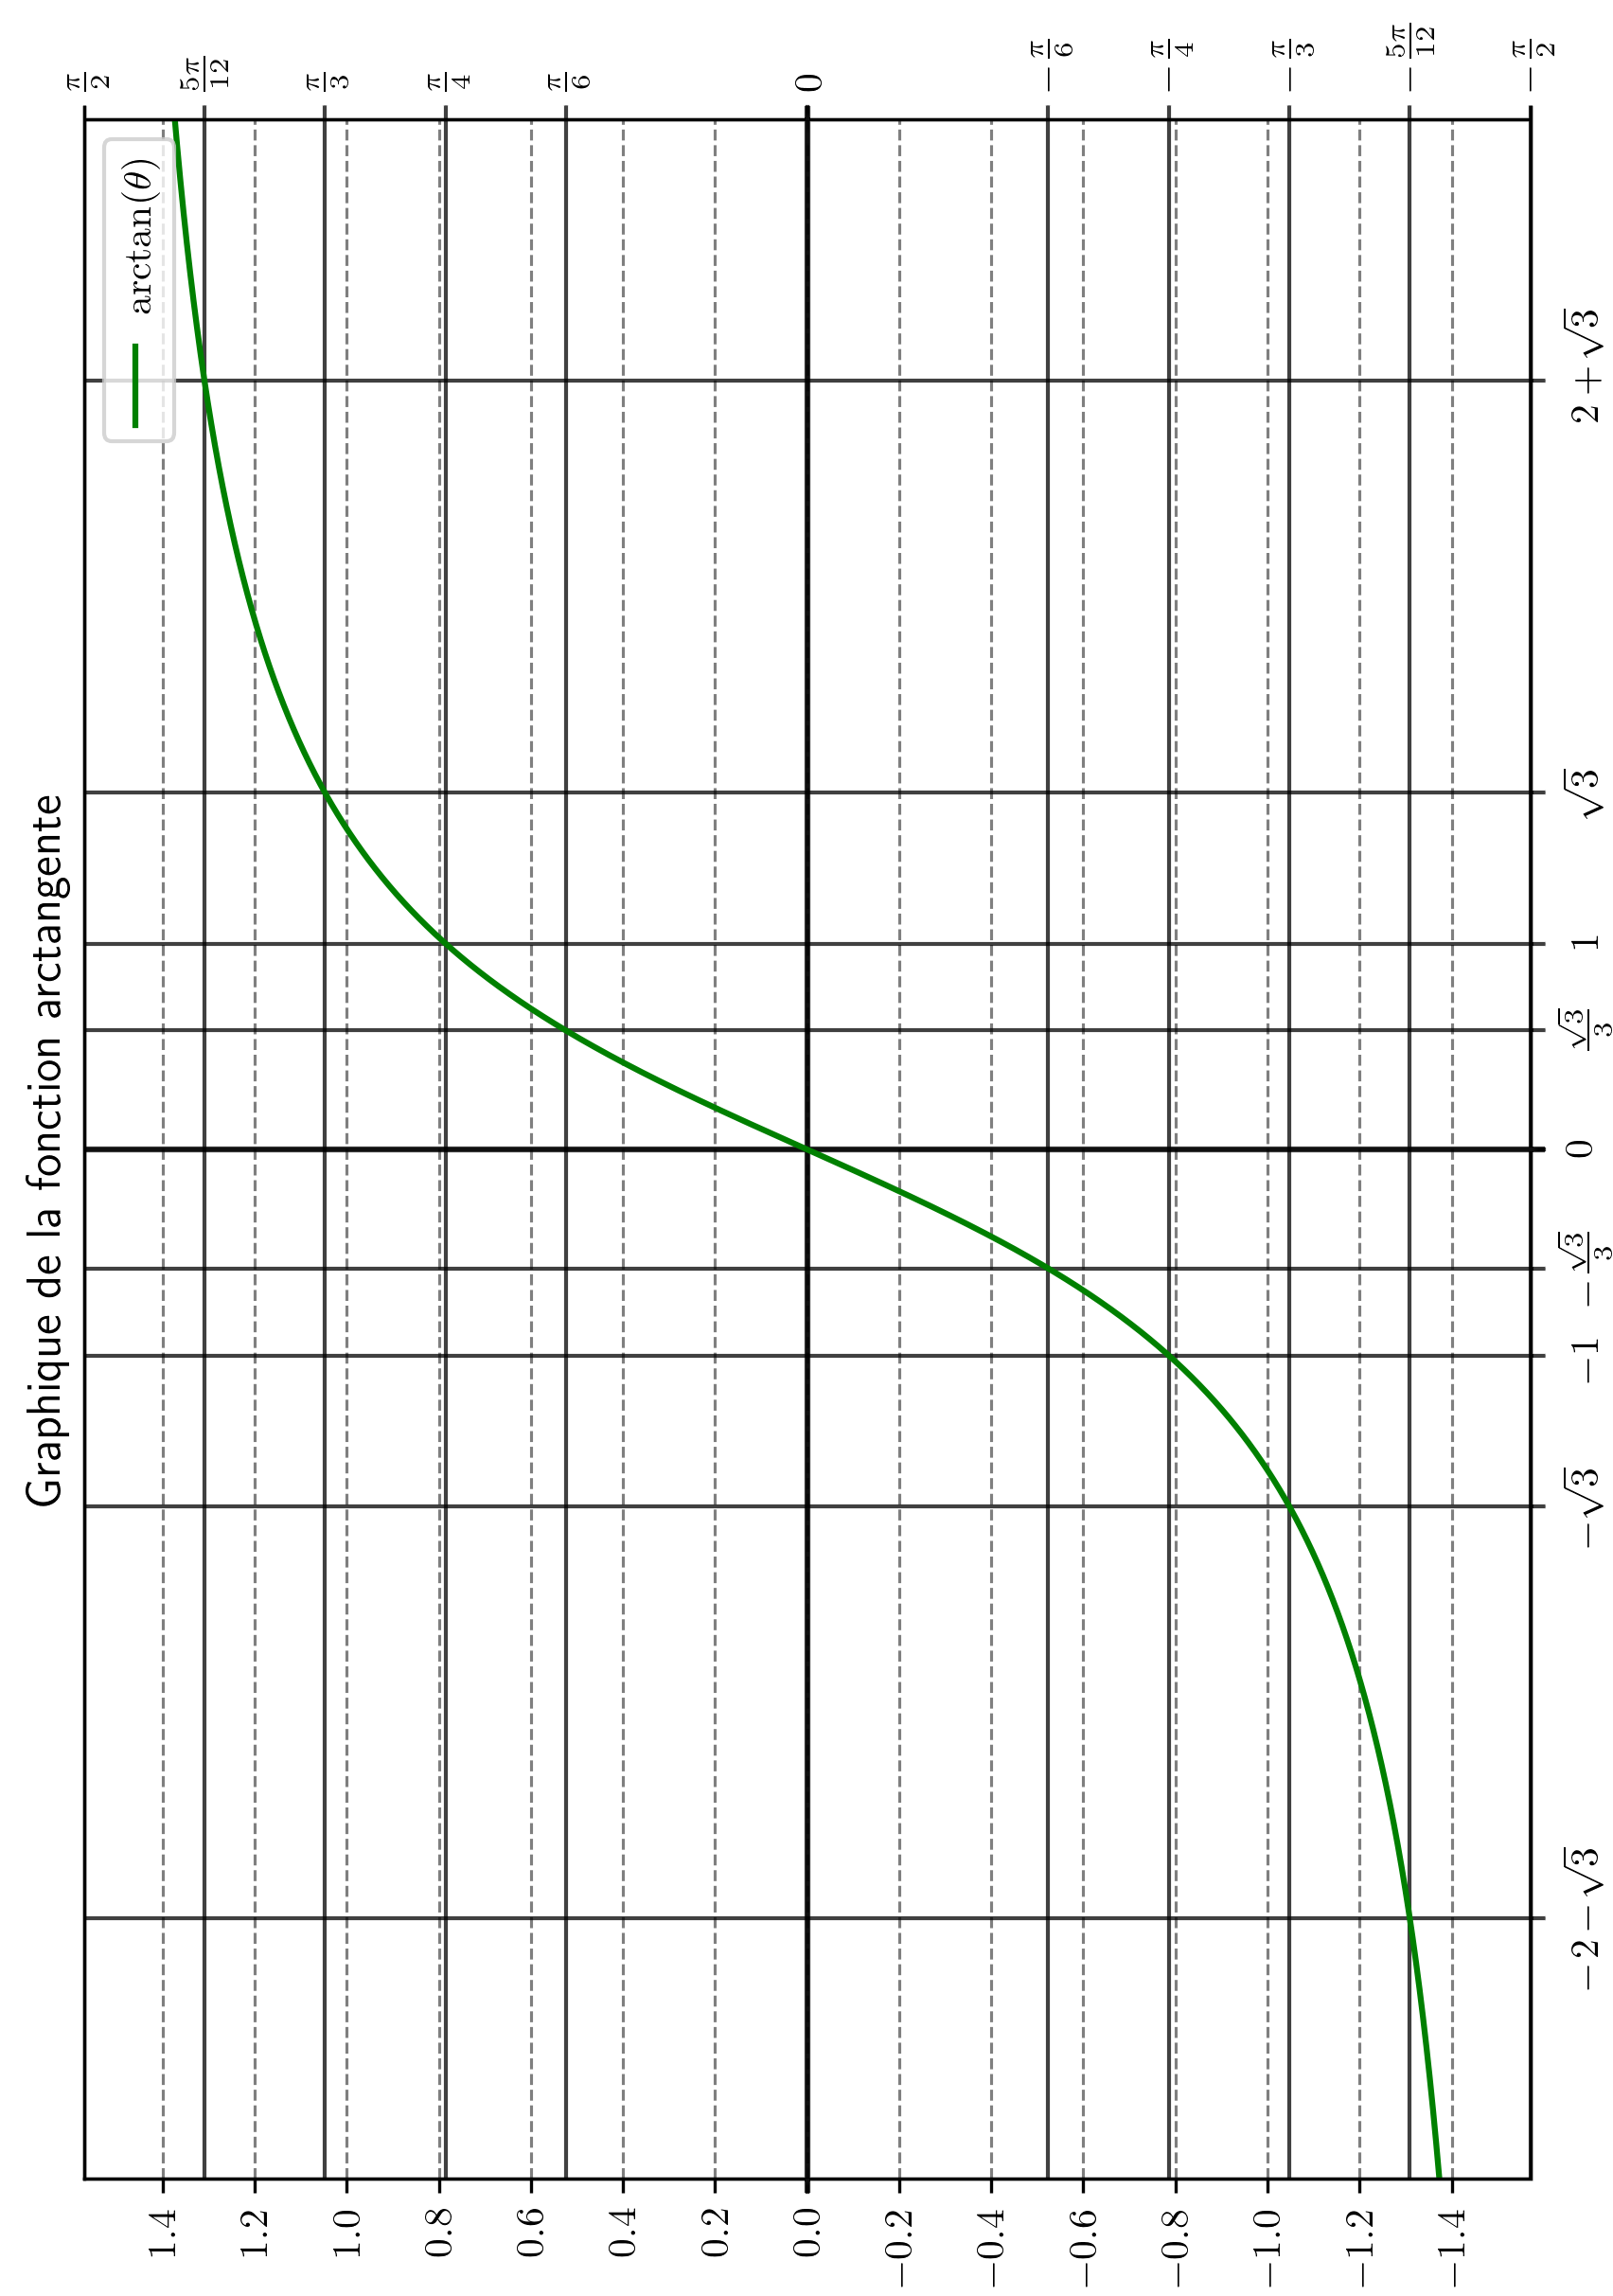
\includegraphics[height=24cm]{Graphs fonctions/arctangente_modifie.png}
				}
			\end{center}

		


			


\newpage

	\section{Formules trigonométriques}

		normalesup.org/~dconduche/prepas/PT/cours/ChapitreFicheTrigo.pdf)

		\subsection*{Définition}

			\setcellgapes{1.5mm}
			\makegapedcells
			\begin{tabular}{ccccc}
				&\multirow{3}{*}{ \Huge{$e^{ix} = \cos x + i \sin x$} }& \\
				$\cos(x) = \frac{e^{ix} + e^{-ix}}{2}$ & $\quad \text{et} \quad$ & $\sin(x) = \frac{e^{ix} - e^{-ix}}{2i}$ & $\quad \text{et} \quad$ & $\tan(x) = \frac{\sin(x)}{\cos(x)}$\\

			\end{tabular}


		
$\cos^2(a) + \sin^2(a) = 1 \quad \text{(On est sur le cercle de rayon 1, d'équation } x^2 + y^2 = 1)$

$\cos(a + b) = \cos(a) \cos(b) - \sin(a) \sin(b)$

$\sin(a + b) = \cos(a) \sin(b) + \sin(a) \cos(b)$

En développant $e^{i(a+b)} = e^{ia} e^{ib}$, puis en identifiant partie réelle et partie imaginaire :

$\tan(a + b) = \frac{\tan(a) + \tan(b)}{1 - \tan(a) \tan(b)}$

En combinant les deux formules précédentes :

$\cos(2a) = \cos^2(a) - \sin^2(a) = 2 \cos^2(a) - 1 = 1 - 2 \sin^2(a) = \frac{1 - \tan^2(a)}{1 + \tan^2(a)}$

$\sin(2a) = 2 \sin(a) \cos(a) = \frac{2 \tan(a)}{1 + \tan^2(a)}$

$\tan(2a) = \frac{2 \tan(a)}{1 - \tan^2(a)}$

$2 \cos(a) \cos(b) = \cos(a + b) + \cos(a - b)$

$2 \sin(a) \sin(b) = -\cos(a + b) + \cos(a - b)$

$2 \sin(a) \cos(b) = \sin(a + b) + \sin(a - b)$

$\cos(a) \cos(b) = \Re \left(e^{ia} \cos(b)\right) = \Re \left(e^{ia} \frac{e^{ib} + e^{-ib}}{2}\right) \quad \text{puis la linéarité de la partie réelle, etc.}$

$\cos(p) + \cos(q) = 2 \cos \left(\frac{p + q}{2}\right) \cos \left(\frac{p - q}{2}\right)$

$-\cos(p) + \cos(q) = 2 \sin \left(\frac{p + q}{2}\right) \sin \left(\frac{p - q}{2}\right)$

$\sin(p) + \sin(q) = 2 \sin \left(\frac{p + q}{2}\right) \cos \left(\frac{p - q}{2}\right)$

Les mêmes que les précédentes, mais dans l'autre sens, avec $p = a + b$ et $q = a - b$.

\section*{Formulaire Trigonométrie Hyperbolique}

En trigonométrie hyperbolique, on suit la même démarche, souvent seuls quelques signes changent devant les $sh$.

$e^x = \cosh x + \sinh x$

$\cosh(x) = \frac{e^x + e^{-x}}{2} \quad \text{et} \quad \sinh(x) = \frac{e^x - e^{-x}}{2}$

$\cosh^2(a) - \sinh^2(a) = 1$

$\cosh(a + b) = \cosh(a) \cosh(b) + \sinh(a) \sinh(b)$

$\sinh(a + b) = \cosh(a) \sinh(b) + \sinh(a) \cosh(b)$

$\tanh(a + b) = \frac{\tanh(a) + \tanh(b)}{1 + \tanh(a) \tanh(b)}$

$\cosh(2a) = \cosh^2(a) + \sinh^2(a) = 2 \cosh^2(a) - 1 = 1 + 2 \sinh^2(a) = \frac{1 + \tanh^2(a)}{1 - \tanh^2(a)}$

$\sinh(2a) = 2 \sinh(a) \cosh(a) = \frac{2 \tanh(a)}{1 - \tanh^2(a)}$

$\tanh(2a) = \frac{2 \tanh(a)}{1 + \tanh^2(a)}$

$2 \cosh(a) \cosh(b) = \cosh(a + b) + \cosh(a - b)$

$2 \sinh(a) \sinh(b) = \cosh(a + b) - \cosh(a - b)$

$2 \sinh(a) \cosh(b) = \sinh(a + b) + \sinh(a - b)$

Se retrouvent à partir des formules de $\cosh(a+b)$, $\cosh(a-b)$, etc. Ou en prenant les parties paires et impaires, sur le modèle de $\Re$ et $\Im$.

$\cosh(p) + \cosh(q) = 2 \cosh \left(\frac{p + q}{2}\right) \cosh \left(\frac{p - q}{2}\right)$

$\cosh(p) - \cosh(q) = 2 \sinh \left(\frac{p + q}{2}\right) \sinh \left(\frac{p - q}{2}\right)$

$\sinh(p) + \sinh(q) = 2 \sinh \left(\frac{p + q}{2}\right) \cosh \left(\frac{p - q}{2}\right)$

Les mêmes que les précédentes, mais dans l'autre sens, avec $p = a + b$ et $q = a - b$.


	\section{Lecture de la table}

	\section{Annexe}

		\subsection*{Fonctions trigonométriques chelous} \label{fonction_trigo_chelous}

		Fonctions trigonométriques chelous selon Github copilot :

		\begin{itemize}
				\item [•] La fonction sinus, notée $\sin$.
				\item [•] La fonction cosinus, notée $\cos$.
				\item [•] La fonction tangente, notée $\tan$.
				\item [•] La fonction cotangente, notée $\cot$.
				\item [•] La fonction sécante, notée $\sec$.
				\item [•] La fonction cosécante, notée $\csc$.
				\item [•] La fonction exsecante, notée $\text{exsec}$.
				\item [•] La fonction excosécante, notée $\text{excsc}$.
				\item [•] La fonction versine, notée $\text{vers}$.
				\item [•] La fonction coversine, notée $\text{covers}$.
				\item [•] La fonction haversine, notée $\text{havers}$.
				\item [•] La fonction hacoversine, notée $\text{hacovers}$.
				\item [•] La fonction exverse, notée $\text{exvers}$.
				\item [•] La fonction excovers, notée $\text{excovers}$.
				\item [•] La fonction vercosine, notée $\text{vercos}$.
				\item [•] La fonction coverscosine, notée $\text{coverscos}$.
				\item [•] La fonction havercosine, notée $\text{havercos}$.
				\item [•] La fonction hacoverscosine, notée $\text{hacoverscos}$.
				\item [•] La fonction exvercosine, notée $\text{exvercos}$.
				\item [•] La fonction excoverscosine, notée $\text{excoverscos}$.
				\item [•] La fonction exsecant, notée $\text{exsec}$.
				\item [•] La fonction excosecant, notée $\text{excsc}$.
				\item [•] La fonction exsecant, notée $\text{exsec}$.
			\end{itemize}

		\subsection*{Valeurs de sinus et cosinus exactes} \label{valeur_remarquable_trigo}

		\subsection*{Démonstration des propriétés des fonctions trigonométrique élémentaires} \label{demo_propriete_trigo_1}



\end{document}